\beginsong{Über meiner Heimat Frühling}[
    wuw={tusk (Eberhard Köbel)}, 
    pfii={91}, 
    pfiii={62}, 
    bo={324}, 
    gruen={11}, 
    kssiv={7}, 
    siru={233},
]

\beginverse
\endverse
\centering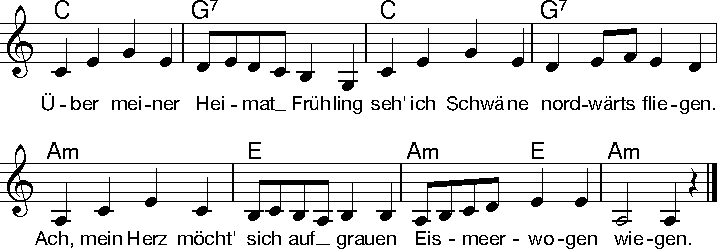
\includegraphics[width=1\textwidth]{Noten/Lied087.pdf}	

\beginverse
\[C]Schwan, im Singsang \[G7]deiner Lieder, \[C]grüß' die grünen \[G7]Birkenhaine.
\[Am]Alle Rosen \[E]gäb' ich gerne \[Am]gegen \[E]Nordlands \[Am]Steine.
\endverse

\beginverse
^Grüße Schweden, ^weißer Vogel! ^Setz an meiner ^statt die Füße
^auf den kalten ^Fels der Ostsee, ^sag' ihr ^meine ^Grüße.
\endverse
\beginverse
^Grüß das Eismeer, ^grüß' das Nordkap! ^Sing den Schären ^zu, den Fjorden,
^wie ein Schwan sei ^meine Seele ^auf dem ^Weg nach ^Norden.
\endverse

\endsong

\beginscripture{}
Hain = Wald; Schäre = kleine Insel (kommen vor allem in Skandinavien vor); Fjord = ins Land reichender Meeresarm
\endscripture
